\documentclass[a4paper,12pt]{article}

\usepackage{amsfonts}
\usepackage[T1]{fontenc}
\usepackage[utf8]{inputenc}
\usepackage{amsmath}
\usepackage{graphicx}

\title{Progettazione del database}

\begin{document}
\maketitle

In questo documento verranno descritte le specifiche e la struttura del database relativo al lato server. Il modello di sviluppo che si vuole seguire è quello di un database relazionale, quindi nella prima sezione verranno mostrate le specifiche, in seguito lo schema entity-relationship e in fine lo schema logico che verrà implementato sul DBMS. 

\section*{Specifiche}
Si vuole descrivere il modello dei dati che devono essere registrati all'interno del database per l'applicazione da sviluppare. Sono di interesse le informazioni di seguito elencate:
\begin{itemize}
\item Gli Utenti di cui si vuole conoscere l'email,che li identifica, e la password con la quale effettuano il login. (Da valutare) Devono essere anche registrati i dati per i pagamenti in-app. Ad ogni Utente possono essere associati più Player.
\item I Player sono gli alter-ego degli Utenti. Ogni Player è associato ad un solo Utente. Per ogni Player deve essere memorizzata anche l'esperienza acquisita durante il gioco e il Livello che ne determina le statistiche insieme alla Classe.
\item Il Livello determina le statistiche base del Player che sono la vita, l'attacco, la difesa e l'esperienza necessaria.
\item La Classe determina i fattori di crescita delle statistiche del Player. La Classe è identificata dal nome. Per ogni Classe sono associate delle Skill.
\item Le Skill sono le abilità speciali associate ad ogni classe, ognuna delle quali è caratterizzata dal nome. Per ogni Skill si deve memorizzare il danno e la frequenza di utilizzo.
\item La base di dati dovrà tenere traccia anche delle Sfide tra i giocatori le quali saranno identificate dai Player coinvolti e l'ora e la data in cui è avvenuto lo scontro. Nelle Sfide deve essere tenuta traccia anche del vincitore della stessa.
\end{itemize} 
\section*{Schema Entity-Relatioship}
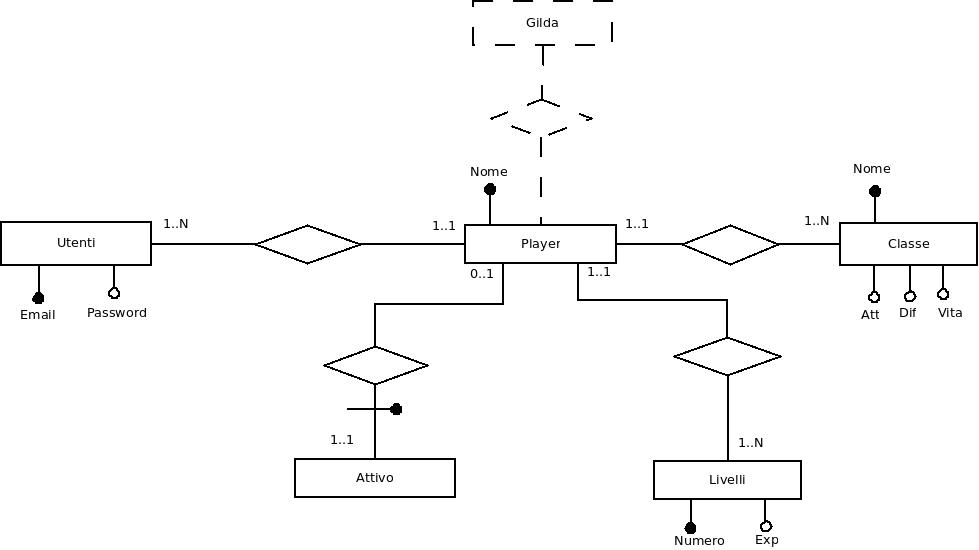
\includegraphics[scale=0.4]{SchemaER.jpeg}

\end{document}